%==============================================================================
% Chapitre 56 - Les bourres
%==============================================================================

\section{Introduction}

La bourre constitue l'un des éléments les plus importants d'une cartouche de
chasse.

Bien que souvent méconnue du grand public, elle influence fortement le
comportement de la munition et la qualité de la gerbe.

\begin{aretenir}

La bourre transmet l'énergie de la poudre à la charge tout en influençant la
dispersion des projectiles.

\end{aretenir}

\section{Position dans la cartouche}

La bourre est située entre la poudre et la charge de projectiles.

Elle constitue l'interface mécanique entre les gaz produits par la combustion
et la charge propulsée.

\begin{figure}[htbp]
\centering

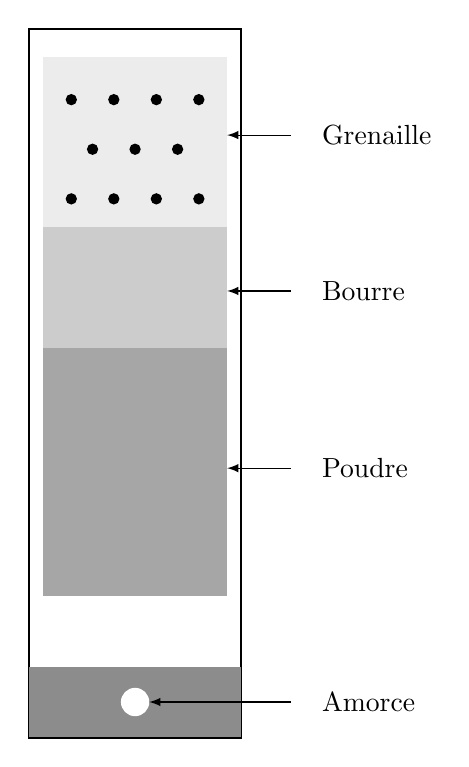
\begin{tikzpicture}[scale=0.9]

% Douille
\draw[thick] (0,0) rectangle (3,10);

% Grenaille
\fill[gray!15] (0.2,7.2) rectangle (2.8,9.6);

\foreach \x/\y in {
0.6/7.6,1.2/7.6,1.8/7.6,2.4/7.6,
0.9/8.3,1.5/8.3,2.1/8.3,
0.6/9.0,1.2/9.0,1.8/9.0,2.4/9.0
}
{
\fill (\x,\y) circle (0.08);
}

% Bourre
\fill[gray!40] (0.2,5.5) rectangle (2.8,7.2);

% Poudre
\fill[gray!70] (0.2,2.0) rectangle (2.8,5.5);

% Culot
\fill[gray!90] (0,0) rectangle (3,1);

% Amorce
\fill[white] (1.5,0.5) circle (0.2);

\node[right] at (4,8.5) {Grenaille};
\node[right] at (4,6.3) {Bourre};
\node[right] at (4,3.8) {Poudre};
\node[right] at (4,0.5) {Amorce};

\draw[-latex] (3.7,8.5) -- (2.8,8.5);
\draw[-latex] (3.7,6.3) -- (2.8,6.3);
\draw[-latex] (3.7,3.8) -- (2.8,3.8);
\draw[-latex] (3.7,0.5) -- (1.7,0.5);

\end{tikzpicture}

\caption{Position de la bourre dans une cartouche de chasse.}
\label{fig:position_bourre}

\end{figure}

\section{Fonctions principales}

La bourre remplit plusieurs fonctions simultanément :

\begin{itemize}
    \item transmettre la poussée ;
    \item assurer l'étanchéité ;
    \item protéger les projectiles ;
    \item influencer la gerbe ;
    \item amortir certaines contraintes mécaniques.
\end{itemize}

\section{Transmission de la poussée}

Lors du tir, les gaz produits par la poudre exercent une pression importante.

La bourre transmet cette pression à la charge de manière efficace.

\section{Étanchéité}

Une bonne étanchéité limite les pertes de gaz.

Elle contribue directement au rendement de la cartouche.

\section{Protection des projectiles}

La bourre protège les projectiles du contact direct avec les parois du canon.

Cette fonction est particulièrement importante avec les bourres modernes à
jupe.

\section{Les bourres traditionnelles}

Pendant longtemps, les bourres étaient réalisées dans des matériaux naturels.

On utilisait notamment :

\begin{itemize}
    \item le feutre ;
    \item le carton ;
    \item le liège ;
    \item certaines fibres végétales.
\end{itemize}

\section{Les bourres grasses}

La bourre grasse est une forme classique de bourre traditionnelle.

Elle est généralement constituée de feutre ou de matériaux similaires.

\section{Les bourres modernes}

Les bourres modernes sont généralement fabriquées en matière synthétique.

Elles offrent des performances plus régulières.

\section{La bourre à jupe}

La bourre à jupe est devenue très répandue.

Elle entoure partiellement la charge de grenaille et limite les contacts avec
le canon.

\begin{figure}[htbp]
\centering

\begin{tikzpicture}

% Bourre grasse
\draw[thick] (0,0) rectangle (2,4);

\node at (1,2) {Feutre};

\node at (1,-0.8)
{Bourre grasse};

% Bourre à jupe
\begin{scope}[xshift=7cm]

\draw[thick] (0.7,0) rectangle (1.3,4);

\draw[thick] (0,2) -- (2,2);

\draw[thick] (0,4) -- (0.7,4);
\draw[thick] (1.3,4) -- (2,4);

\node at (1,-0.8)
{Bourre à jupe};

\end{scope}

\end{tikzpicture}

\caption{Comparaison simplifiée entre une bourre grasse et une bourre à jupe.}
\label{fig:bourre_grasse_jupe}

\end{figure}

\section{Protection de la gerbe}

En limitant les déformations des projectiles, la bourre à jupe contribue à
maintenir une gerbe plus homogène.

\begin{figure}[htbp]
\centering

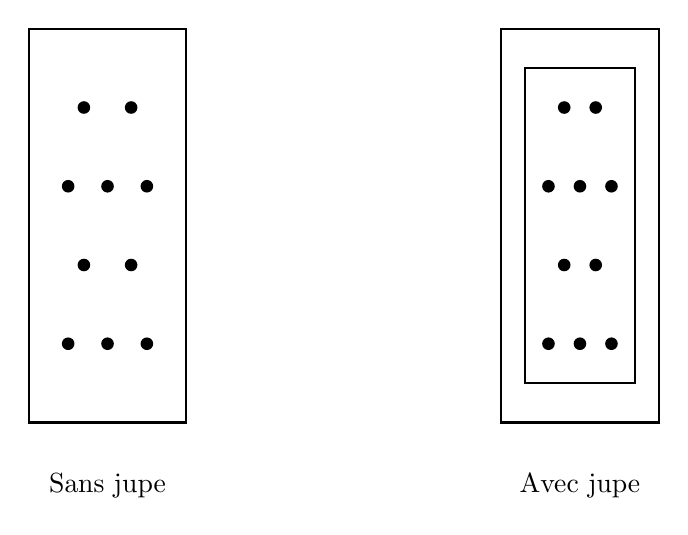
\begin{tikzpicture}[scale=1]

% Sans jupe
\draw[thick] (0,0) rectangle (2,5);

\foreach \x/\y in {
0.5/1,1.0/1,1.5/1,
0.7/2,1.3/2,
0.5/3,1.0/3,1.5/3,
0.7/4,1.3/4
}
{
\fill (\x,\y) circle (0.08);
}

\node at (1,-0.8) {Sans jupe};

% Avec jupe
\begin{scope}[xshift=6cm]

\draw[thick] (0,0) rectangle (2,5);

\draw[thick] (0.3,0.5) rectangle (1.7,4.5);

\foreach \x/\y in {
0.6/1,1.0/1,1.4/1,
0.8/2,1.2/2,
0.6/3,1.0/3,1.4/3,
0.8/4,1.2/4
}
{
\fill (\x,\y) circle (0.08);
}

\node at (1,-0.8) {Avec jupe};

\end{scope}

\end{tikzpicture}

\caption{La bourre à jupe limite le contact direct entre la grenaille et le canon.}
\label{fig:protection_grenaille}

\end{figure}

\section{Séparation après la bouche}

Après la sortie du canon, la bourre poursuit brièvement sa trajectoire.

Elle se sépare ensuite de la charge de projectiles.

\begin{figure}[htbp]
\centering

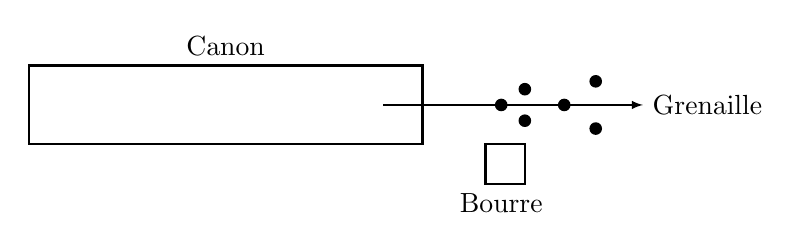
\begin{tikzpicture}[scale=1]

% Canon
\draw[thick] (0,1) rectangle (5,2);

\node[above] at (2.5,2)
{Canon};

% Charge
\foreach \x/\y in {
6/1.5,
6.3/1.7,
6.3/1.3,
6.8/1.5,
7.2/1.8,
7.2/1.2
}
{
\fill (\x,\y) circle (0.08);
}

% Bourre
\draw[thick]
(5.8,0.5)
rectangle
(6.3,1.0);

% Flèches
\draw[-latex] (4.5,1.5) -- (7.8,1.5);

\node[right] at (7.8,1.5)
{Grenaille};

\node[below] at (6.0,0.5)
{Bourre};

\end{tikzpicture}

\caption{Après la sortie du canon, la bourre se sépare progressivement de la charge.}
\label{fig:separation_bourre}

\end{figure}

\section{Influence sur la dispersion}

La conception de la bourre influence directement :

\begin{itemize}
    \item la densité de la gerbe ;
    \item la régularité des impacts ;
    \item la dispersion.
\end{itemize}

\section{Compatibilité avec les chokes}

Le comportement de la bourre dépend également du choke utilisé.

L'interaction entre ces deux éléments influence fortement les résultats en
cible.

\section{Applications selon le type de chasse}

Certaines bourres sont privilégiées pour les tirs à courte distance.

D'autres sont davantage adaptées aux tirs plus lointains.

Le choix dépend donc de l'usage recherché.

\section{Évolution des matériaux}

Les préoccupations environnementales ont conduit au développement de nouvelles
solutions.

Les matériaux utilisés continuent d'évoluer.

\section{Vers les chokes}

La bourre influence fortement la gerbe, mais elle n'est pas le seul élément en
cause.

Le chapitre suivant présentera les chokes et leur rôle dans le contrôle de la
dispersion.

\begin{figure}[htbp]
\centering

\begin{tikzpicture}

% Bourre grasse
\node at (0,4) {Bourre grasse};

\draw[dashed] (0,0) ellipse (2.2 and 1.3);

\foreach \x/\y in {
-1.2/0.6,-0.7/0.9,0.1/0.5,1.1/0.6,
-1.3/-0.5,-0.2/-0.8,0.9/-0.6,
0.0/0.0,0.6/0.1,-0.6/0.2
}
{
\fill (\x,\y) circle (0.06);
}

% Bourre à jupe
\begin{scope}[xshift=8cm]

\node at (0,4) {Bourre à jupe};

\draw[dashed] (0,0) ellipse (1.2 and 0.8);

\foreach \x/\y in {
-0.4/0.2,-0.2/0.4,0.0/0.1,
0.3/0.3,0.5/0.0,-0.3/-0.2,
0.2/-0.3,0.0/0.0,0.4/-0.1,
-0.5/0.0
}
{
\fill (\x,\y) circle (0.06);
}

\end{scope}

\end{tikzpicture}

\caption{Influence simplifiée de la bourre sur la dispersion de la gerbe.}
\label{fig:influence_bourre_gerbe}

\end{figure}

\section{À retenir}

\begin{aretenir}

\begin{itemize}
    \item La bourre assure plusieurs fonctions simultanément.
    \item Elle transmet la poussée des gaz à la charge.
    \item Les bourres à jupe protègent efficacement les projectiles.
    \item La bourre influence directement la gerbe.
    \item Son comportement dépend également du choke utilisé.
\end{itemize}

\end{aretenir}
